
% Default to the notebook output style

    


% Inherit from the specified cell style.




    
\documentclass[11pt]{article}

    
    
    \usepackage[T1]{fontenc}
    % Nicer default font (+ math font) than Computer Modern for most use cases
    \usepackage{mathpazo}

    % Basic figure setup, for now with no caption control since it's done
    % automatically by Pandoc (which extracts ![](path) syntax from Markdown).
    \usepackage{graphicx}
    % We will generate all images so they have a width \maxwidth. This means
    % that they will get their normal width if they fit onto the page, but
    % are scaled down if they would overflow the margins.
    \makeatletter
    \def\maxwidth{\ifdim\Gin@nat@width>\linewidth\linewidth
    \else\Gin@nat@width\fi}
    \makeatother
    \let\Oldincludegraphics\includegraphics
    % Set max figure width to be 80% of text width, for now hardcoded.
    \renewcommand{\includegraphics}[1]{\Oldincludegraphics[width=.8\maxwidth]{#1}}
    % Ensure that by default, figures have no caption (until we provide a
    % proper Figure object with a Caption API and a way to capture that
    % in the conversion process - todo).
    \usepackage{caption}
    \DeclareCaptionLabelFormat{nolabel}{}
    \captionsetup{labelformat=nolabel}

    \usepackage{adjustbox} % Used to constrain images to a maximum size 
    \usepackage{xcolor} % Allow colors to be defined
    \usepackage{enumerate} % Needed for markdown enumerations to work
    \usepackage{geometry} % Used to adjust the document margins
    \usepackage{amsmath} % Equations
    \usepackage{amssymb} % Equations
    \usepackage{textcomp} % defines textquotesingle
    % Hack from http://tex.stackexchange.com/a/47451/13684:
    \AtBeginDocument{%
        \def\PYZsq{\textquotesingle}% Upright quotes in Pygmentized code
    }
    \usepackage{upquote} % Upright quotes for verbatim code
    \usepackage{eurosym} % defines \euro
    \usepackage[mathletters]{ucs} % Extended unicode (utf-8) support
    \usepackage[utf8x]{inputenc} % Allow utf-8 characters in the tex document
    \usepackage{fancyvrb} % verbatim replacement that allows latex
    \usepackage{grffile} % extends the file name processing of package graphics 
                         % to support a larger range 
    % The hyperref package gives us a pdf with properly built
    % internal navigation ('pdf bookmarks' for the table of contents,
    % internal cross-reference links, web links for URLs, etc.)
    \usepackage{hyperref}
    \usepackage{longtable} % longtable support required by pandoc >1.10
    \usepackage{booktabs}  % table support for pandoc > 1.12.2
    \usepackage[inline]{enumitem} % IRkernel/repr support (it uses the enumerate* environment)
    \usepackage[normalem]{ulem} % ulem is needed to support strikethroughs (\sout)
                                % normalem makes italics be italics, not underlines
    

    
    
    % Colors for the hyperref package
    \definecolor{urlcolor}{rgb}{0,.145,.698}
    \definecolor{linkcolor}{rgb}{.71,0.21,0.01}
    \definecolor{citecolor}{rgb}{.12,.54,.11}

    % ANSI colors
    \definecolor{ansi-black}{HTML}{3E424D}
    \definecolor{ansi-black-intense}{HTML}{282C36}
    \definecolor{ansi-red}{HTML}{E75C58}
    \definecolor{ansi-red-intense}{HTML}{B22B31}
    \definecolor{ansi-green}{HTML}{00A250}
    \definecolor{ansi-green-intense}{HTML}{007427}
    \definecolor{ansi-yellow}{HTML}{DDB62B}
    \definecolor{ansi-yellow-intense}{HTML}{B27D12}
    \definecolor{ansi-blue}{HTML}{208FFB}
    \definecolor{ansi-blue-intense}{HTML}{0065CA}
    \definecolor{ansi-magenta}{HTML}{D160C4}
    \definecolor{ansi-magenta-intense}{HTML}{A03196}
    \definecolor{ansi-cyan}{HTML}{60C6C8}
    \definecolor{ansi-cyan-intense}{HTML}{258F8F}
    \definecolor{ansi-white}{HTML}{C5C1B4}
    \definecolor{ansi-white-intense}{HTML}{A1A6B2}

    % commands and environments needed by pandoc snippets
    % extracted from the output of `pandoc -s`
    \providecommand{\tightlist}{%
      \setlength{\itemsep}{0pt}\setlength{\parskip}{0pt}}
    \DefineVerbatimEnvironment{Highlighting}{Verbatim}{commandchars=\\\{\}}
    % Add ',fontsize=\small' for more characters per line
    \newenvironment{Shaded}{}{}
    \newcommand{\KeywordTok}[1]{\textcolor[rgb]{0.00,0.44,0.13}{\textbf{{#1}}}}
    \newcommand{\DataTypeTok}[1]{\textcolor[rgb]{0.56,0.13,0.00}{{#1}}}
    \newcommand{\DecValTok}[1]{\textcolor[rgb]{0.25,0.63,0.44}{{#1}}}
    \newcommand{\BaseNTok}[1]{\textcolor[rgb]{0.25,0.63,0.44}{{#1}}}
    \newcommand{\FloatTok}[1]{\textcolor[rgb]{0.25,0.63,0.44}{{#1}}}
    \newcommand{\CharTok}[1]{\textcolor[rgb]{0.25,0.44,0.63}{{#1}}}
    \newcommand{\StringTok}[1]{\textcolor[rgb]{0.25,0.44,0.63}{{#1}}}
    \newcommand{\CommentTok}[1]{\textcolor[rgb]{0.38,0.63,0.69}{\textit{{#1}}}}
    \newcommand{\OtherTok}[1]{\textcolor[rgb]{0.00,0.44,0.13}{{#1}}}
    \newcommand{\AlertTok}[1]{\textcolor[rgb]{1.00,0.00,0.00}{\textbf{{#1}}}}
    \newcommand{\FunctionTok}[1]{\textcolor[rgb]{0.02,0.16,0.49}{{#1}}}
    \newcommand{\RegionMarkerTok}[1]{{#1}}
    \newcommand{\ErrorTok}[1]{\textcolor[rgb]{1.00,0.00,0.00}{\textbf{{#1}}}}
    \newcommand{\NormalTok}[1]{{#1}}
    
    % Additional commands for more recent versions of Pandoc
    \newcommand{\ConstantTok}[1]{\textcolor[rgb]{0.53,0.00,0.00}{{#1}}}
    \newcommand{\SpecialCharTok}[1]{\textcolor[rgb]{0.25,0.44,0.63}{{#1}}}
    \newcommand{\VerbatimStringTok}[1]{\textcolor[rgb]{0.25,0.44,0.63}{{#1}}}
    \newcommand{\SpecialStringTok}[1]{\textcolor[rgb]{0.73,0.40,0.53}{{#1}}}
    \newcommand{\ImportTok}[1]{{#1}}
    \newcommand{\DocumentationTok}[1]{\textcolor[rgb]{0.73,0.13,0.13}{\textit{{#1}}}}
    \newcommand{\AnnotationTok}[1]{\textcolor[rgb]{0.38,0.63,0.69}{\textbf{\textit{{#1}}}}}
    \newcommand{\CommentVarTok}[1]{\textcolor[rgb]{0.38,0.63,0.69}{\textbf{\textit{{#1}}}}}
    \newcommand{\VariableTok}[1]{\textcolor[rgb]{0.10,0.09,0.49}{{#1}}}
    \newcommand{\ControlFlowTok}[1]{\textcolor[rgb]{0.00,0.44,0.13}{\textbf{{#1}}}}
    \newcommand{\OperatorTok}[1]{\textcolor[rgb]{0.40,0.40,0.40}{{#1}}}
    \newcommand{\BuiltInTok}[1]{{#1}}
    \newcommand{\ExtensionTok}[1]{{#1}}
    \newcommand{\PreprocessorTok}[1]{\textcolor[rgb]{0.74,0.48,0.00}{{#1}}}
    \newcommand{\AttributeTok}[1]{\textcolor[rgb]{0.49,0.56,0.16}{{#1}}}
    \newcommand{\InformationTok}[1]{\textcolor[rgb]{0.38,0.63,0.69}{\textbf{\textit{{#1}}}}}
    \newcommand{\WarningTok}[1]{\textcolor[rgb]{0.38,0.63,0.69}{\textbf{\textit{{#1}}}}}
    
    
    % Define a nice break command that doesn't care if a line doesn't already
    % exist.
    \def\br{\hspace*{\fill} \\* }
    % Math Jax compatability definitions
    \def\gt{>}
    \def\lt{<}
    % Document parameters
    \title{sheet1}
    
    
    

    % Pygments definitions
    
\makeatletter
\def\PY@reset{\let\PY@it=\relax \let\PY@bf=\relax%
    \let\PY@ul=\relax \let\PY@tc=\relax%
    \let\PY@bc=\relax \let\PY@ff=\relax}
\def\PY@tok#1{\csname PY@tok@#1\endcsname}
\def\PY@toks#1+{\ifx\relax#1\empty\else%
    \PY@tok{#1}\expandafter\PY@toks\fi}
\def\PY@do#1{\PY@bc{\PY@tc{\PY@ul{%
    \PY@it{\PY@bf{\PY@ff{#1}}}}}}}
\def\PY#1#2{\PY@reset\PY@toks#1+\relax+\PY@do{#2}}

\expandafter\def\csname PY@tok@w\endcsname{\def\PY@tc##1{\textcolor[rgb]{0.73,0.73,0.73}{##1}}}
\expandafter\def\csname PY@tok@c\endcsname{\let\PY@it=\textit\def\PY@tc##1{\textcolor[rgb]{0.25,0.50,0.50}{##1}}}
\expandafter\def\csname PY@tok@cp\endcsname{\def\PY@tc##1{\textcolor[rgb]{0.74,0.48,0.00}{##1}}}
\expandafter\def\csname PY@tok@k\endcsname{\let\PY@bf=\textbf\def\PY@tc##1{\textcolor[rgb]{0.00,0.50,0.00}{##1}}}
\expandafter\def\csname PY@tok@kp\endcsname{\def\PY@tc##1{\textcolor[rgb]{0.00,0.50,0.00}{##1}}}
\expandafter\def\csname PY@tok@kt\endcsname{\def\PY@tc##1{\textcolor[rgb]{0.69,0.00,0.25}{##1}}}
\expandafter\def\csname PY@tok@o\endcsname{\def\PY@tc##1{\textcolor[rgb]{0.40,0.40,0.40}{##1}}}
\expandafter\def\csname PY@tok@ow\endcsname{\let\PY@bf=\textbf\def\PY@tc##1{\textcolor[rgb]{0.67,0.13,1.00}{##1}}}
\expandafter\def\csname PY@tok@nb\endcsname{\def\PY@tc##1{\textcolor[rgb]{0.00,0.50,0.00}{##1}}}
\expandafter\def\csname PY@tok@nf\endcsname{\def\PY@tc##1{\textcolor[rgb]{0.00,0.00,1.00}{##1}}}
\expandafter\def\csname PY@tok@nc\endcsname{\let\PY@bf=\textbf\def\PY@tc##1{\textcolor[rgb]{0.00,0.00,1.00}{##1}}}
\expandafter\def\csname PY@tok@nn\endcsname{\let\PY@bf=\textbf\def\PY@tc##1{\textcolor[rgb]{0.00,0.00,1.00}{##1}}}
\expandafter\def\csname PY@tok@ne\endcsname{\let\PY@bf=\textbf\def\PY@tc##1{\textcolor[rgb]{0.82,0.25,0.23}{##1}}}
\expandafter\def\csname PY@tok@nv\endcsname{\def\PY@tc##1{\textcolor[rgb]{0.10,0.09,0.49}{##1}}}
\expandafter\def\csname PY@tok@no\endcsname{\def\PY@tc##1{\textcolor[rgb]{0.53,0.00,0.00}{##1}}}
\expandafter\def\csname PY@tok@nl\endcsname{\def\PY@tc##1{\textcolor[rgb]{0.63,0.63,0.00}{##1}}}
\expandafter\def\csname PY@tok@ni\endcsname{\let\PY@bf=\textbf\def\PY@tc##1{\textcolor[rgb]{0.60,0.60,0.60}{##1}}}
\expandafter\def\csname PY@tok@na\endcsname{\def\PY@tc##1{\textcolor[rgb]{0.49,0.56,0.16}{##1}}}
\expandafter\def\csname PY@tok@nt\endcsname{\let\PY@bf=\textbf\def\PY@tc##1{\textcolor[rgb]{0.00,0.50,0.00}{##1}}}
\expandafter\def\csname PY@tok@nd\endcsname{\def\PY@tc##1{\textcolor[rgb]{0.67,0.13,1.00}{##1}}}
\expandafter\def\csname PY@tok@s\endcsname{\def\PY@tc##1{\textcolor[rgb]{0.73,0.13,0.13}{##1}}}
\expandafter\def\csname PY@tok@sd\endcsname{\let\PY@it=\textit\def\PY@tc##1{\textcolor[rgb]{0.73,0.13,0.13}{##1}}}
\expandafter\def\csname PY@tok@si\endcsname{\let\PY@bf=\textbf\def\PY@tc##1{\textcolor[rgb]{0.73,0.40,0.53}{##1}}}
\expandafter\def\csname PY@tok@se\endcsname{\let\PY@bf=\textbf\def\PY@tc##1{\textcolor[rgb]{0.73,0.40,0.13}{##1}}}
\expandafter\def\csname PY@tok@sr\endcsname{\def\PY@tc##1{\textcolor[rgb]{0.73,0.40,0.53}{##1}}}
\expandafter\def\csname PY@tok@ss\endcsname{\def\PY@tc##1{\textcolor[rgb]{0.10,0.09,0.49}{##1}}}
\expandafter\def\csname PY@tok@sx\endcsname{\def\PY@tc##1{\textcolor[rgb]{0.00,0.50,0.00}{##1}}}
\expandafter\def\csname PY@tok@m\endcsname{\def\PY@tc##1{\textcolor[rgb]{0.40,0.40,0.40}{##1}}}
\expandafter\def\csname PY@tok@gh\endcsname{\let\PY@bf=\textbf\def\PY@tc##1{\textcolor[rgb]{0.00,0.00,0.50}{##1}}}
\expandafter\def\csname PY@tok@gu\endcsname{\let\PY@bf=\textbf\def\PY@tc##1{\textcolor[rgb]{0.50,0.00,0.50}{##1}}}
\expandafter\def\csname PY@tok@gd\endcsname{\def\PY@tc##1{\textcolor[rgb]{0.63,0.00,0.00}{##1}}}
\expandafter\def\csname PY@tok@gi\endcsname{\def\PY@tc##1{\textcolor[rgb]{0.00,0.63,0.00}{##1}}}
\expandafter\def\csname PY@tok@gr\endcsname{\def\PY@tc##1{\textcolor[rgb]{1.00,0.00,0.00}{##1}}}
\expandafter\def\csname PY@tok@ge\endcsname{\let\PY@it=\textit}
\expandafter\def\csname PY@tok@gs\endcsname{\let\PY@bf=\textbf}
\expandafter\def\csname PY@tok@gp\endcsname{\let\PY@bf=\textbf\def\PY@tc##1{\textcolor[rgb]{0.00,0.00,0.50}{##1}}}
\expandafter\def\csname PY@tok@go\endcsname{\def\PY@tc##1{\textcolor[rgb]{0.53,0.53,0.53}{##1}}}
\expandafter\def\csname PY@tok@gt\endcsname{\def\PY@tc##1{\textcolor[rgb]{0.00,0.27,0.87}{##1}}}
\expandafter\def\csname PY@tok@err\endcsname{\def\PY@bc##1{\setlength{\fboxsep}{0pt}\fcolorbox[rgb]{1.00,0.00,0.00}{1,1,1}{\strut ##1}}}
\expandafter\def\csname PY@tok@kc\endcsname{\let\PY@bf=\textbf\def\PY@tc##1{\textcolor[rgb]{0.00,0.50,0.00}{##1}}}
\expandafter\def\csname PY@tok@kd\endcsname{\let\PY@bf=\textbf\def\PY@tc##1{\textcolor[rgb]{0.00,0.50,0.00}{##1}}}
\expandafter\def\csname PY@tok@kn\endcsname{\let\PY@bf=\textbf\def\PY@tc##1{\textcolor[rgb]{0.00,0.50,0.00}{##1}}}
\expandafter\def\csname PY@tok@kr\endcsname{\let\PY@bf=\textbf\def\PY@tc##1{\textcolor[rgb]{0.00,0.50,0.00}{##1}}}
\expandafter\def\csname PY@tok@bp\endcsname{\def\PY@tc##1{\textcolor[rgb]{0.00,0.50,0.00}{##1}}}
\expandafter\def\csname PY@tok@fm\endcsname{\def\PY@tc##1{\textcolor[rgb]{0.00,0.00,1.00}{##1}}}
\expandafter\def\csname PY@tok@vc\endcsname{\def\PY@tc##1{\textcolor[rgb]{0.10,0.09,0.49}{##1}}}
\expandafter\def\csname PY@tok@vg\endcsname{\def\PY@tc##1{\textcolor[rgb]{0.10,0.09,0.49}{##1}}}
\expandafter\def\csname PY@tok@vi\endcsname{\def\PY@tc##1{\textcolor[rgb]{0.10,0.09,0.49}{##1}}}
\expandafter\def\csname PY@tok@vm\endcsname{\def\PY@tc##1{\textcolor[rgb]{0.10,0.09,0.49}{##1}}}
\expandafter\def\csname PY@tok@sa\endcsname{\def\PY@tc##1{\textcolor[rgb]{0.73,0.13,0.13}{##1}}}
\expandafter\def\csname PY@tok@sb\endcsname{\def\PY@tc##1{\textcolor[rgb]{0.73,0.13,0.13}{##1}}}
\expandafter\def\csname PY@tok@sc\endcsname{\def\PY@tc##1{\textcolor[rgb]{0.73,0.13,0.13}{##1}}}
\expandafter\def\csname PY@tok@dl\endcsname{\def\PY@tc##1{\textcolor[rgb]{0.73,0.13,0.13}{##1}}}
\expandafter\def\csname PY@tok@s2\endcsname{\def\PY@tc##1{\textcolor[rgb]{0.73,0.13,0.13}{##1}}}
\expandafter\def\csname PY@tok@sh\endcsname{\def\PY@tc##1{\textcolor[rgb]{0.73,0.13,0.13}{##1}}}
\expandafter\def\csname PY@tok@s1\endcsname{\def\PY@tc##1{\textcolor[rgb]{0.73,0.13,0.13}{##1}}}
\expandafter\def\csname PY@tok@mb\endcsname{\def\PY@tc##1{\textcolor[rgb]{0.40,0.40,0.40}{##1}}}
\expandafter\def\csname PY@tok@mf\endcsname{\def\PY@tc##1{\textcolor[rgb]{0.40,0.40,0.40}{##1}}}
\expandafter\def\csname PY@tok@mh\endcsname{\def\PY@tc##1{\textcolor[rgb]{0.40,0.40,0.40}{##1}}}
\expandafter\def\csname PY@tok@mi\endcsname{\def\PY@tc##1{\textcolor[rgb]{0.40,0.40,0.40}{##1}}}
\expandafter\def\csname PY@tok@il\endcsname{\def\PY@tc##1{\textcolor[rgb]{0.40,0.40,0.40}{##1}}}
\expandafter\def\csname PY@tok@mo\endcsname{\def\PY@tc##1{\textcolor[rgb]{0.40,0.40,0.40}{##1}}}
\expandafter\def\csname PY@tok@ch\endcsname{\let\PY@it=\textit\def\PY@tc##1{\textcolor[rgb]{0.25,0.50,0.50}{##1}}}
\expandafter\def\csname PY@tok@cm\endcsname{\let\PY@it=\textit\def\PY@tc##1{\textcolor[rgb]{0.25,0.50,0.50}{##1}}}
\expandafter\def\csname PY@tok@cpf\endcsname{\let\PY@it=\textit\def\PY@tc##1{\textcolor[rgb]{0.25,0.50,0.50}{##1}}}
\expandafter\def\csname PY@tok@c1\endcsname{\let\PY@it=\textit\def\PY@tc##1{\textcolor[rgb]{0.25,0.50,0.50}{##1}}}
\expandafter\def\csname PY@tok@cs\endcsname{\let\PY@it=\textit\def\PY@tc##1{\textcolor[rgb]{0.25,0.50,0.50}{##1}}}

\def\PYZbs{\char`\\}
\def\PYZus{\char`\_}
\def\PYZob{\char`\{}
\def\PYZcb{\char`\}}
\def\PYZca{\char`\^}
\def\PYZam{\char`\&}
\def\PYZlt{\char`\<}
\def\PYZgt{\char`\>}
\def\PYZsh{\char`\#}
\def\PYZpc{\char`\%}
\def\PYZdl{\char`\$}
\def\PYZhy{\char`\-}
\def\PYZsq{\char`\'}
\def\PYZdq{\char`\"}
\def\PYZti{\char`\~}
% for compatibility with earlier versions
\def\PYZat{@}
\def\PYZlb{[}
\def\PYZrb{]}
\makeatother


    % Exact colors from NB
    \definecolor{incolor}{rgb}{0.0, 0.0, 0.5}
    \definecolor{outcolor}{rgb}{0.545, 0.0, 0.0}



    
    % Prevent overflowing lines due to hard-to-break entities
    \sloppy 
    % Setup hyperref package
    \hypersetup{
      breaklinks=true,  % so long urls are correctly broken across lines
      colorlinks=true,
      urlcolor=urlcolor,
      linkcolor=linkcolor,
      citecolor=citecolor,
      }
    % Slightly bigger margins than the latex defaults
    
    \geometry{verbose,tmargin=1in,bmargin=1in,lmargin=1in,rmargin=1in}
    
    

    \begin{document}
    
    
    \maketitle
    
    

    
    \section{Deep Neural Networks: Forward and Backward
Propagation}\label{deep-neural-networks-forward-and-backward-propagation}

In this homework, our goal is to test different approaches to program
neural networks, from the simplest and least general one to the most
complex and general. Here, we will be focusing on programming forward
and gradient computations. Training neural networks will be left for
Homework 2. The first implementation we consider is a hard-coded neural
network made of one input layer, three hidden layers, and one output
layer. We use the ReLU nonlinearity at each hidden layer. The neural
network is depicted below:

\begin{figure}
\centering
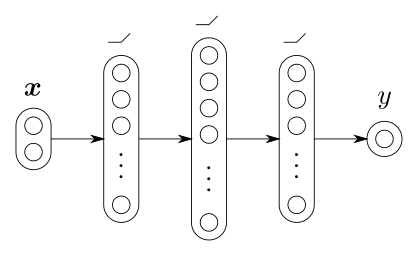
\includegraphics{net.svg.png}
\caption{}
\end{figure}

The following implementation performs forward and gradient computations
using \textbf{\texttt{for}} loops. The code is compact but only works
for this specific architecture. It is hard to extend it to new layers
without significantly refactoring and complexifying the code.

    \begin{Verbatim}[commandchars=\\\{\}]
{\color{incolor}In [{\color{incolor}1}]:} \PY{k+kn}{import} \PY{n+nn}{numpy}\PY{o}{,}\PY{n+nn}{numpy}\PY{n+nn}{.}\PY{n+nn}{linalg}
        
        \PY{k}{def} \PY{n+nf}{implementation1}\PY{p}{(}\PY{n}{X}\PY{p}{,}\PY{n}{T}\PY{p}{,}\PY{n}{W}\PY{p}{,}\PY{n}{B}\PY{p}{)}\PY{p}{:}
        
            \PY{c+c1}{\PYZsh{} 1. Initialize some data structures}
            \PY{n}{A}\PY{p}{,}\PY{n}{Z} \PY{o}{=} \PY{p}{[}\PY{n}{X}\PY{p}{]}\PY{p}{,}\PY{p}{[}\PY{p}{]}
            \PY{n}{DW}\PY{p}{,}\PY{n}{DB} \PY{o}{=} \PY{p}{[}\PY{p}{]}\PY{p}{,}\PY{p}{[}\PY{p}{]}
        
            \PY{c+c1}{\PYZsh{} 2. Run the forward pass}
            \PY{k}{for} \PY{n}{i}\PY{p}{,}\PY{p}{(}\PY{n}{w}\PY{p}{,}\PY{n}{b}\PY{p}{)} \PY{o+ow}{in} \PY{n+nb}{enumerate}\PY{p}{(}\PY{n+nb}{zip}\PY{p}{(}\PY{n}{W}\PY{p}{,}\PY{n}{B}\PY{p}{)}\PY{p}{)}\PY{p}{:}
                \PY{n}{Z}\PY{o}{.}\PY{n}{append}\PY{p}{(}\PY{n}{A}\PY{p}{[}\PY{o}{\PYZhy{}}\PY{l+m+mi}{1}\PY{p}{]}\PY{o}{.}\PY{n}{dot}\PY{p}{(}\PY{n}{w}\PY{p}{)}\PY{o}{+}\PY{n}{b}\PY{p}{)}
                \PY{k}{if} \PY{n}{i} \PY{o+ow}{in} \PY{p}{[}\PY{l+m+mi}{0}\PY{p}{,}\PY{l+m+mi}{1}\PY{p}{,}\PY{l+m+mi}{2}\PY{p}{]}\PY{p}{:} \PY{n}{A}\PY{o}{.}\PY{n}{append}\PY{p}{(}\PY{n}{numpy}\PY{o}{.}\PY{n}{maximum}\PY{p}{(}\PY{l+m+mi}{0}\PY{p}{,}\PY{n}{Z}\PY{p}{[}\PY{o}{\PYZhy{}}\PY{l+m+mi}{1}\PY{p}{]}\PY{p}{)}\PY{p}{)}
            \PY{n}{Y} \PY{o}{=} \PY{n}{Z}\PY{p}{[}\PY{o}{\PYZhy{}}\PY{l+m+mi}{1}\PY{p}{]}
        
            \PY{c+c1}{\PYZsh{} 3. Compute the error}
            \PY{n}{Y} \PY{o}{=} \PY{n}{Z}\PY{p}{[}\PY{o}{\PYZhy{}}\PY{l+m+mi}{1}\PY{p}{]}
            \PY{n}{err} \PY{o}{=} \PY{p}{(}\PY{p}{(}\PY{n}{Y}\PY{o}{\PYZhy{}}\PY{n}{T}\PY{p}{)}\PY{o}{*}\PY{o}{*}\PY{l+m+mi}{2}\PY{p}{)}\PY{o}{.}\PY{n}{mean}\PY{p}{(}\PY{p}{)}
            \PY{n}{grad} \PY{o}{=} \PY{l+m+mi}{2}\PY{o}{*}\PY{p}{(}\PY{n}{Y}\PY{o}{\PYZhy{}}\PY{n}{T}\PY{p}{)}
        
            \PY{c+c1}{\PYZsh{} 4. Gradient propagation}
            \PY{k}{for} \PY{n}{w}\PY{p}{,}\PY{n}{b}\PY{p}{,}\PY{n}{a} \PY{o+ow}{in} \PY{n+nb}{zip}\PY{p}{(}\PY{n}{W}\PY{p}{[}\PY{p}{:}\PY{p}{:}\PY{o}{\PYZhy{}}\PY{l+m+mi}{1}\PY{p}{]}\PY{p}{,}\PY{n}{B}\PY{p}{[}\PY{p}{:}\PY{p}{:}\PY{o}{\PYZhy{}}\PY{l+m+mi}{1}\PY{p}{]}\PY{p}{,}\PY{n}{A}\PY{p}{[}\PY{p}{:}\PY{p}{:}\PY{o}{\PYZhy{}}\PY{l+m+mi}{1}\PY{p}{]}\PY{p}{)}\PY{p}{:}
                \PY{n}{DW}\PY{o}{.}\PY{n}{insert}\PY{p}{(}\PY{l+m+mi}{0}\PY{p}{,}\PY{n}{a}\PY{o}{.}\PY{n}{T}\PY{o}{.}\PY{n}{dot}\PY{p}{(}\PY{n}{grad}\PY{p}{)}\PY{o}{/}\PY{n+nb}{len}\PY{p}{(}\PY{n}{a}\PY{p}{)}\PY{p}{)}
                \PY{n}{DB}\PY{o}{.}\PY{n}{insert}\PY{p}{(}\PY{l+m+mi}{0}\PY{p}{,}\PY{n}{grad}\PY{o}{.}\PY{n}{mean}\PY{p}{(}\PY{n}{axis}\PY{o}{=}\PY{l+m+mi}{0}\PY{p}{)}\PY{p}{)}
                \PY{n}{grad} \PY{o}{=} \PY{n}{grad}\PY{o}{.}\PY{n}{dot}\PY{p}{(}\PY{n}{w}\PY{o}{.}\PY{n}{T}\PY{p}{)}\PY{o}{*}\PY{p}{(}\PY{n}{a}\PY{o}{\PYZgt{}}\PY{l+m+mi}{0}\PY{p}{)}
        
            \PY{c+c1}{\PYZsh{} 5. Return error and gradient}
            \PY{k}{return} \PY{n}{err}\PY{p}{,}\PY{n}{DW}
\end{Verbatim}


    The code below applies this function to a given dataset \texttt{X,T} at
a given position \texttt{W,B} in parameter space, where these two
variables contain the weight and bias parameters at each layer. It then
prints the prediction mean square error, and the gradient norm at each
layer.

    \begin{Verbatim}[commandchars=\\\{\}]
{\color{incolor}In [{\color{incolor}2}]:} \PY{k+kn}{import} \PY{n+nn}{utils}
        
        \PY{n}{X}\PY{p}{,}\PY{n}{T} \PY{o}{=} \PY{n}{utils}\PY{o}{.}\PY{n}{getdata}\PY{p}{(}\PY{l+m+mi}{100}\PY{p}{)}
        \PY{n}{W}\PY{p}{,}\PY{n}{B} \PY{o}{=} \PY{n}{utils}\PY{o}{.}\PY{n}{getparameters}\PY{p}{(}\PY{p}{[}\PY{n}{X}\PY{o}{.}\PY{n}{shape}\PY{p}{[}\PY{l+m+mi}{1}\PY{p}{]}\PY{p}{,}\PY{l+m+mi}{10}\PY{p}{,}\PY{l+m+mi}{15}\PY{p}{,}\PY{l+m+mi}{10}\PY{p}{,}\PY{n}{T}\PY{o}{.}\PY{n}{shape}\PY{p}{[}\PY{l+m+mi}{1}\PY{p}{]}\PY{p}{]}\PY{p}{)}
        
        \PY{n}{err}\PY{p}{,}\PY{n}{DW} \PY{o}{=} \PY{n}{implementation1}\PY{p}{(}\PY{n}{X}\PY{p}{,}\PY{n}{T}\PY{p}{,}\PY{n}{W}\PY{p}{,}\PY{n}{B}\PY{p}{)}
        
        \PY{n+nb}{print}\PY{p}{(}\PY{n}{err}\PY{p}{,}\PY{n+nb}{map}\PY{p}{(}\PY{n}{numpy}\PY{o}{.}\PY{n}{linalg}\PY{o}{.}\PY{n}{norm}\PY{p}{,}\PY{n}{DW}\PY{p}{)}\PY{p}{)}
\end{Verbatim}


    \begin{Verbatim}[commandchars=\\\{\}]
(1.1593903177325451, [0.29622485370120832, 0.6949589001193901, 1.3754967914824301, 0.80223630277879099])

    \end{Verbatim}

    These numbers are not specially interesting (the network has not been
trained), however, they are useful for debugging purposes, in order to
verify that the next implementations work as expected.

\subsection{Object-Oriented Implementation (15
P)}\label{object-oriented-implementation-15-p}

The following implmentation adopts an object oriented approach to the
forward and gradient computations. Each layer is an object with methods
implementing the forward and backward pass for this layer. Objects are
defined in the file \texttt{layers.py}. Overall, the code is longer, but
it is better structured and easier to extend.

    \begin{Verbatim}[commandchars=\\\{\}]
{\color{incolor}In [{\color{incolor}3}]:} \PY{k+kn}{import} \PY{n+nn}{layers}
            
        \PY{k}{def} \PY{n+nf}{implementation2}\PY{p}{(}\PY{n}{X}\PY{p}{,}\PY{n}{T}\PY{p}{,}\PY{n}{W}\PY{p}{,}\PY{n}{B}\PY{p}{,}\PY{n}{NonLin}\PY{p}{)}\PY{p}{:}
            
            \PY{c+c1}{\PYZsh{} 1. Build the neural network}
            \PY{n}{nnlayers} \PY{o}{=} \PY{p}{[}\PY{p}{]}
            \PY{k}{for} \PY{n}{w}\PY{p}{,}\PY{n}{b} \PY{o+ow}{in} \PY{n+nb}{zip}\PY{p}{(}\PY{n}{W}\PY{p}{,}\PY{n}{B}\PY{p}{)}\PY{p}{:} \PY{n}{nnlayers} \PY{o}{+}\PY{o}{=} \PY{p}{[}\PY{n}{layers}\PY{o}{.}\PY{n}{Linear}\PY{p}{(}\PY{n}{w}\PY{p}{,}\PY{n}{b}\PY{p}{)}\PY{p}{]} \PY{o}{+} \PY{p}{(}\PY{p}{[}\PY{n}{NonLin}\PY{p}{(}\PY{p}{)}\PY{p}{]} \PY{k}{if} \PY{n+nb}{len}\PY{p}{(}\PY{n}{b}\PY{p}{)}\PY{o}{!=}\PY{l+m+mi}{1} \PY{k}{else} \PY{p}{[}\PY{p}{]}\PY{p}{)}
            \PY{n}{nn} \PY{o}{=} \PY{n}{layers}\PY{o}{.}\PY{n}{Sequential}\PY{p}{(}\PY{n}{nnlayers}\PY{p}{)}
        
            \PY{c+c1}{\PYZsh{} 2. Compute the error and its gradient}
            \PY{n}{Y} \PY{o}{=} \PY{n}{nn}\PY{o}{.}\PY{n}{forward}\PY{p}{(}\PY{n}{X}\PY{p}{)}
            \PY{n}{err} \PY{o}{=} \PY{p}{(}\PY{p}{(}\PY{n}{Y}\PY{o}{\PYZhy{}}\PY{n}{T}\PY{p}{)}\PY{o}{*}\PY{o}{*}\PY{l+m+mi}{2}\PY{p}{)}\PY{o}{.}\PY{n}{mean}\PY{p}{(}\PY{p}{)}
            \PY{n}{nn}\PY{o}{.}\PY{n}{backward}\PY{p}{(}\PY{l+m+mi}{2}\PY{o}{*}\PY{p}{(}\PY{n}{Y}\PY{o}{\PYZhy{}}\PY{n}{T}\PY{p}{)}\PY{p}{)}
        
            \PY{c+c1}{\PYZsh{} 3. Return them}
            \PY{k}{return} \PY{n}{err}\PY{p}{,}\PY{p}{[}\PY{n}{nn}\PY{o}{.}\PY{n}{layers}\PY{p}{[}\PY{n}{i}\PY{p}{]}\PY{o}{.}\PY{n}{DW} \PY{k}{for} \PY{n}{i} \PY{o+ow}{in} \PY{p}{[}\PY{l+m+mi}{0}\PY{p}{,}\PY{l+m+mi}{2}\PY{p}{,}\PY{l+m+mi}{4}\PY{p}{,}\PY{l+m+mi}{6}\PY{p}{]}\PY{p}{]}
            
\end{Verbatim}


    The code below computes and prints the prediction error, and the
gradient norm at each layer.

    \begin{Verbatim}[commandchars=\\\{\}]
{\color{incolor}In [{\color{incolor}4}]:} \PY{k+kn}{import} \PY{n+nn}{utils}
        
        \PY{n}{err}\PY{p}{,}\PY{n}{DW} \PY{o}{=} \PY{n}{implementation2}\PY{p}{(}\PY{n}{X}\PY{p}{,}\PY{n}{T}\PY{p}{,}\PY{n}{W}\PY{p}{,}\PY{n}{B}\PY{p}{,}\PY{n}{layers}\PY{o}{.}\PY{n}{Tanh}\PY{p}{)}
        \PY{n+nb}{print}\PY{p}{(}\PY{n}{err}\PY{p}{,}\PY{n+nb}{map}\PY{p}{(}\PY{n}{numpy}\PY{o}{.}\PY{n}{linalg}\PY{o}{.}\PY{n}{norm}\PY{p}{,}\PY{n}{DW}\PY{p}{)}\PY{p}{)}
\end{Verbatim}


    \begin{Verbatim}[commandchars=\\\{\}]
(1.0609541173391692, [0.24642012799448015, 0.49094047912050492, 0.66230622343522649, 0.47314564399410192])

    \end{Verbatim}

    Here, although the data and parameters have not been changed, the
numbers are different as for \texttt{implementation1}, as we have now
made use of the \texttt{Tanh} nonlinearity instead of \texttt{ReLU}.

\textbf{Tasks:}

\begin{itemize}
\tightlist
\item
  \textbf{Define a new layer \texttt{ReLU} to be used in replacement to
  the \texttt{Tanh} layer. This makes the architecture equivalent to the
  neural network implemented by the function \texttt{implementation1}.}
\item
  \textbf{Run the code below to verify that the error and gradient are
  indeed the same for \texttt{implementation1} and
  \texttt{implementation2}.}
\end{itemize}

    \begin{Verbatim}[commandchars=\\\{\}]
{\color{incolor}In [{\color{incolor}6}]:} \PY{k}{class} \PY{n+nc}{ReLU}\PY{p}{:}
            
            \PY{k}{def} \PY{n+nf}{forward}\PY{p}{(}\PY{n+nb+bp}{self}\PY{p}{,}\PY{n}{Z}\PY{p}{)}\PY{p}{:} \PY{n+nb+bp}{self}\PY{o}{.}\PY{n}{A} \PY{o}{=} \PY{n}{numpy}\PY{o}{.}\PY{n}{maximum}\PY{p}{(}\PY{l+m+mi}{0}\PY{p}{,}\PY{n}{Z}\PY{p}{)}\PY{p}{;} \PY{k}{return} \PY{n+nb+bp}{self}\PY{o}{.}\PY{n}{A}
            \PY{k}{def} \PY{n+nf}{backward}\PY{p}{(}\PY{n+nb+bp}{self}\PY{p}{,}\PY{n}{DA}\PY{p}{)}\PY{p}{:} \PY{k}{return} \PY{p}{(}\PY{n+nb+bp}{self}\PY{o}{.}\PY{n}{A}\PY{o}{\PYZgt{}}\PY{l+m+mi}{0}\PY{p}{)}\PY{o}{*}\PY{n}{DA} 
        
        \PY{n}{err}\PY{p}{,}\PY{n}{DW} \PY{o}{=} \PY{n}{implementation1}\PY{p}{(}\PY{n}{X}\PY{p}{,}\PY{n}{T}\PY{p}{,}\PY{n}{W}\PY{p}{,}\PY{n}{B}\PY{p}{)}\PY{p}{;}      \PY{n+nb}{print}\PY{p}{(}\PY{n}{err}\PY{p}{,}\PY{n+nb}{map}\PY{p}{(}\PY{n}{numpy}\PY{o}{.}\PY{n}{linalg}\PY{o}{.}\PY{n}{norm}\PY{p}{,}\PY{n}{DW}\PY{p}{)}\PY{p}{)}
        \PY{n}{err}\PY{p}{,}\PY{n}{DW} \PY{o}{=} \PY{n}{implementation2}\PY{p}{(}\PY{n}{X}\PY{p}{,}\PY{n}{T}\PY{p}{,}\PY{n}{W}\PY{p}{,}\PY{n}{B}\PY{p}{,}\PY{n}{ReLU}\PY{p}{)}\PY{p}{;} \PY{n+nb}{print}\PY{p}{(}\PY{n}{err}\PY{p}{,}\PY{n+nb}{map}\PY{p}{(}\PY{n}{numpy}\PY{o}{.}\PY{n}{linalg}\PY{o}{.}\PY{n}{norm}\PY{p}{,}\PY{n}{DW}\PY{p}{)}\PY{p}{)}
\end{Verbatim}


    \begin{Verbatim}[commandchars=\\\{\}]
(1.1593903177325451, [0.29622485370120832, 0.6949589001193901, 1.3754967914824301, 0.80223630277879099])
(1.1593903177325451, [0.29622485370120832, 0.6949589001193901, 1.3754967914824301, 0.80223630277879099])

    \end{Verbatim}

    \subsection{Implementation for General Graphs (15
P)}\label{implementation-for-general-graphs-15-p}

The implementation below is more complex but is also applicable to a
broader set of structures than simple feed-forward network. Here, the
neural network can be seen as a set of nodes (defined in
\texttt{nodes.py}) that are organized in a graph. Prediction and
computation of gradients are obtained by traversing the graph using
recursion.

    \begin{Verbatim}[commandchars=\\\{\}]
{\color{incolor}In [{\color{incolor}7}]:} \PY{k+kn}{import} \PY{n+nn}{nodes}
            
        \PY{k}{def} \PY{n+nf}{implementation3}\PY{p}{(}\PY{n}{X}\PY{p}{,}\PY{n}{T}\PY{p}{,}\PY{n}{W}\PY{p}{,}\PY{n}{B}\PY{p}{)}\PY{p}{:}
        
            \PY{c+c1}{\PYZsh{} 1. Build the neural network}
            \PY{n}{W}\PY{p}{,}\PY{n}{B} \PY{o}{=} \PY{n}{utils}\PY{o}{.}\PY{n}{getparameters}\PY{p}{(}\PY{p}{[}\PY{n}{X}\PY{o}{.}\PY{n}{shape}\PY{p}{[}\PY{l+m+mi}{1}\PY{p}{]}\PY{p}{,}\PY{l+m+mi}{10}\PY{p}{,}\PY{l+m+mi}{15}\PY{p}{,}\PY{l+m+mi}{10}\PY{p}{,}\PY{n}{T}\PY{o}{.}\PY{n}{shape}\PY{p}{[}\PY{l+m+mi}{1}\PY{p}{]}\PY{p}{]}\PY{p}{)}
        
            \PY{n}{nodeX} \PY{o}{=} \PY{n}{nodes}\PY{o}{.}\PY{n}{Input}\PY{p}{(}\PY{p}{)}
            \PY{n}{nodeA} \PY{o}{=} \PY{n}{nodeX}
            \PY{n}{nodesW} \PY{o}{=} \PY{p}{[}\PY{n}{nodes}\PY{o}{.}\PY{n}{Weight}\PY{p}{(}\PY{n}{w}\PY{p}{)} \PY{k}{for} \PY{n}{w} \PY{o+ow}{in} \PY{n}{W}\PY{p}{]}
            \PY{n}{nodesB} \PY{o}{=} \PY{p}{[}\PY{n}{nodes}\PY{o}{.}\PY{n}{Bias}\PY{p}{(}\PY{n}{b}\PY{p}{)} \PY{k}{for} \PY{n}{b} \PY{o+ow}{in} \PY{n}{B}\PY{p}{]}
        
            \PY{k}{for} \PY{n}{i}\PY{p}{,}\PY{p}{(}\PY{n}{nodeW}\PY{p}{,}\PY{n}{nodeB}\PY{p}{)} \PY{o+ow}{in} \PY{n+nb}{enumerate}\PY{p}{(}\PY{n+nb}{zip}\PY{p}{(}\PY{n}{nodesW}\PY{p}{,}\PY{n}{nodesB}\PY{p}{)}\PY{p}{)}\PY{p}{:}
                \PY{n}{nodeZ} \PY{o}{=} \PY{n}{nodes}\PY{o}{.}\PY{n}{Linear}\PY{p}{(}\PY{n}{nodeA}\PY{p}{,}\PY{n}{nodeW}\PY{p}{,}\PY{n}{nodeB}\PY{p}{)}
                \PY{k}{if} \PY{n}{i} \PY{o+ow}{in} \PY{p}{[}\PY{l+m+mi}{0}\PY{p}{,}\PY{l+m+mi}{1}\PY{p}{,}\PY{l+m+mi}{2}\PY{p}{]}\PY{p}{:} \PY{n}{nodeA} \PY{o}{=} \PY{n}{nodes}\PY{o}{.}\PY{n}{Tanh}\PY{p}{(}\PY{n}{nodeZ}\PY{p}{)}
            \PY{n}{nodeY} \PY{o}{=} \PY{n}{nodes}\PY{o}{.}\PY{n}{Output}\PY{p}{(}\PY{n}{nodeZ}\PY{p}{)}
        
            \PY{c+c1}{\PYZsh{} 2. Compute the error and its gradient}
            \PY{n}{nodeX}\PY{o}{.}\PY{n}{feed}\PY{p}{(}\PY{n}{X}\PY{p}{)}
            \PY{n}{Y} \PY{o}{=} \PY{n}{nodeY}\PY{o}{.}\PY{n}{evaluate}\PY{p}{(}\PY{p}{)}
            \PY{n}{err} \PY{o}{=} \PY{p}{(}\PY{p}{(}\PY{n}{Y}\PY{o}{\PYZhy{}}\PY{n}{T}\PY{p}{)}\PY{o}{*}\PY{o}{*}\PY{l+m+mi}{2}\PY{p}{)}\PY{o}{.}\PY{n}{mean}\PY{p}{(}\PY{p}{)}
            \PY{n}{nodeY}\PY{o}{.}\PY{n}{feed}\PY{p}{(}\PY{l+m+mi}{2}\PY{o}{*}\PY{p}{(}\PY{n}{Y}\PY{o}{\PYZhy{}}\PY{n}{T}\PY{p}{)}\PY{p}{)}
            
            \PY{c+c1}{\PYZsh{} 3. Return them}
            \PY{k}{return} \PY{n}{err}\PY{p}{,}\PY{p}{[}\PY{n}{nodeW}\PY{o}{.}\PY{n}{grad}\PY{p}{(}\PY{p}{)} \PY{k}{for} \PY{n}{nodeW} \PY{o+ow}{in} \PY{n}{nodesW}\PY{p}{]}
\end{Verbatim}


    The code below applies the new implementation on the same dataset and
parameters as before, and the error and gradients are compared for
correctness to those of \texttt{implementation2}.

    \begin{Verbatim}[commandchars=\\\{\}]
{\color{incolor}In [{\color{incolor}8}]:} \PY{n}{err}\PY{p}{,}\PY{n}{DW} \PY{o}{=} \PY{n}{implementation2}\PY{p}{(}\PY{n}{X}\PY{p}{,}\PY{n}{T}\PY{p}{,}\PY{n}{W}\PY{p}{,}\PY{n}{B}\PY{p}{,}\PY{n}{layers}\PY{o}{.}\PY{n}{Tanh}\PY{p}{)}\PY{p}{;} \PY{n+nb}{print}\PY{p}{(}\PY{n}{err}\PY{p}{,}\PY{n+nb}{map}\PY{p}{(}\PY{n}{numpy}\PY{o}{.}\PY{n}{linalg}\PY{o}{.}\PY{n}{norm}\PY{p}{,}\PY{n}{DW}\PY{p}{)}\PY{p}{)}
        \PY{n}{err}\PY{p}{,}\PY{n}{DW} \PY{o}{=} \PY{n}{implementation3}\PY{p}{(}\PY{n}{X}\PY{p}{,}\PY{n}{T}\PY{p}{,}\PY{n}{W}\PY{p}{,}\PY{n}{B}\PY{p}{)}\PY{p}{;}             \PY{n+nb}{print}\PY{p}{(}\PY{n}{err}\PY{p}{,}\PY{n+nb}{map}\PY{p}{(}\PY{n}{numpy}\PY{o}{.}\PY{n}{linalg}\PY{o}{.}\PY{n}{norm}\PY{p}{,}\PY{n}{DW}\PY{p}{)}\PY{p}{)}
\end{Verbatim}


    \begin{Verbatim}[commandchars=\\\{\}]
(1.0609541173391692, [0.24642012799448015, 0.49094047912050492, 0.66230622343522649, 0.47314564399410192])
(1.0609541173391692, [0.24642012799448015, 0.49094047912050492, 0.66230622343522649, 0.47314564399410192])

    \end{Verbatim}

    We now would like to modify the neural network architecture by including
a shortcut connection. Shortcut connections can be useful when the
prediction requires a combination of simple and more abstract features.

\begin{figure}
\centering
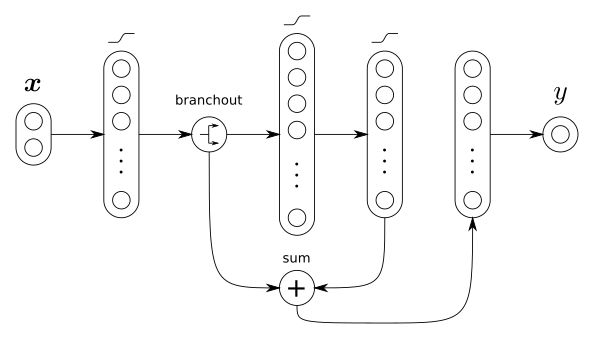
\includegraphics{net-shortcut.svg.png}
\caption{}
\end{figure}

The implementation below assumes two types of nodes, \texttt{Sum} and
\texttt{BranchOut}. Both are needed to implement the network above.

    \begin{Verbatim}[commandchars=\\\{\}]
{\color{incolor}In [{\color{incolor}9}]:} \PY{k}{def} \PY{n+nf}{implementation3B}\PY{p}{(}\PY{n}{X}\PY{p}{,}\PY{n}{T}\PY{p}{,}\PY{n}{W}\PY{p}{,}\PY{n}{B}\PY{p}{,}\PY{n}{Sum}\PY{p}{,}\PY{n}{BranchOut}\PY{p}{)}\PY{p}{:}
            
            \PY{c+c1}{\PYZsh{} 1. Build the neural network}
            \PY{n}{W}\PY{p}{,}\PY{n}{B} \PY{o}{=} \PY{n}{utils}\PY{o}{.}\PY{n}{getparameters}\PY{p}{(}\PY{p}{[}\PY{n}{X}\PY{o}{.}\PY{n}{shape}\PY{p}{[}\PY{l+m+mi}{1}\PY{p}{]}\PY{p}{,}\PY{l+m+mi}{10}\PY{p}{,}\PY{l+m+mi}{15}\PY{p}{,}\PY{l+m+mi}{10}\PY{p}{,}\PY{n}{T}\PY{o}{.}\PY{n}{shape}\PY{p}{[}\PY{l+m+mi}{1}\PY{p}{]}\PY{p}{]}\PY{p}{)}
        
            \PY{n}{nodeX} \PY{o}{=} \PY{n}{nodes}\PY{o}{.}\PY{n}{Input}\PY{p}{(}\PY{p}{)}
            \PY{n}{nodesW} \PY{o}{=} \PY{p}{[}\PY{n}{nodes}\PY{o}{.}\PY{n}{Weight}\PY{p}{(}\PY{n}{w}\PY{p}{)} \PY{k}{for} \PY{n}{w} \PY{o+ow}{in} \PY{n}{W}\PY{p}{]}
            \PY{n}{nodesB} \PY{o}{=} \PY{p}{[}\PY{n}{nodes}\PY{o}{.}\PY{n}{Bias}\PY{p}{(}\PY{n}{b}\PY{p}{)} \PY{k}{for} \PY{n}{b} \PY{o+ow}{in} \PY{n}{B}\PY{p}{]}
        
            \PY{n}{nodeZ1} \PY{o}{=} \PY{n}{nodes}\PY{o}{.}\PY{n}{Linear}\PY{p}{(}\PY{n}{nodeX}\PY{p}{,}\PY{n}{nodesW}\PY{p}{[}\PY{l+m+mi}{0}\PY{p}{]}\PY{p}{,}\PY{n}{nodesB}\PY{p}{[}\PY{l+m+mi}{0}\PY{p}{]}\PY{p}{)}
            \PY{n}{nodeA1} \PY{o}{=} \PY{n}{nodes}\PY{o}{.}\PY{n}{Tanh}\PY{p}{(}\PY{n}{nodeZ1}\PY{p}{)}
            \PY{n}{nodeQ1} \PY{o}{=} \PY{n}{BranchOut}\PY{p}{(}\PY{n}{nodeA1}\PY{p}{)}
        
            \PY{n}{nodeZ2} \PY{o}{=} \PY{n}{nodes}\PY{o}{.}\PY{n}{Linear}\PY{p}{(}\PY{n}{nodeQ1}\PY{p}{,}\PY{n}{nodesW}\PY{p}{[}\PY{l+m+mi}{1}\PY{p}{]}\PY{p}{,}\PY{n}{nodesB}\PY{p}{[}\PY{l+m+mi}{1}\PY{p}{]}\PY{p}{)}
            \PY{n}{nodeA2} \PY{o}{=} \PY{n}{nodes}\PY{o}{.}\PY{n}{Tanh}\PY{p}{(}\PY{n}{nodeZ2}\PY{p}{)}
            \PY{n}{nodeZ3} \PY{o}{=} \PY{n}{nodes}\PY{o}{.}\PY{n}{Linear}\PY{p}{(}\PY{n}{nodeA2}\PY{p}{,}\PY{n}{nodesW}\PY{p}{[}\PY{l+m+mi}{2}\PY{p}{]}\PY{p}{,}\PY{n}{nodesB}\PY{p}{[}\PY{l+m+mi}{2}\PY{p}{]}\PY{p}{)}
            \PY{n}{nodeA3} \PY{o}{=} \PY{n}{nodes}\PY{o}{.}\PY{n}{Tanh}\PY{p}{(}\PY{n}{nodeZ3}\PY{p}{)}
            \PY{n}{nodeS3} \PY{o}{=} \PY{n}{Sum}\PY{p}{(}\PY{p}{[}\PY{n}{nodeQ1}\PY{p}{,}\PY{n}{nodeA3}\PY{p}{]}\PY{p}{)}
        
            \PY{n}{nodeZ4} \PY{o}{=} \PY{n}{nodes}\PY{o}{.}\PY{n}{Linear}\PY{p}{(}\PY{n}{nodeS3}\PY{p}{,}\PY{n}{nodesW}\PY{p}{[}\PY{l+m+mi}{3}\PY{p}{]}\PY{p}{,}\PY{n}{nodesB}\PY{p}{[}\PY{l+m+mi}{3}\PY{p}{]}\PY{p}{)}
            \PY{n}{nodeOut} \PY{o}{=} \PY{n}{nodes}\PY{o}{.}\PY{n}{Output}\PY{p}{(}\PY{n}{nodeZ4}\PY{p}{)}
        
            \PY{c+c1}{\PYZsh{} 2. Compute the error and its gradient}
            \PY{n}{nodeX}\PY{o}{.}\PY{n}{feed}\PY{p}{(}\PY{n}{X}\PY{p}{)}
            \PY{n}{Y} \PY{o}{=} \PY{n}{nodeOut}\PY{o}{.}\PY{n}{evaluate}\PY{p}{(}\PY{p}{)}
            \PY{n}{err} \PY{o}{=} \PY{p}{(}\PY{p}{(}\PY{n}{Y}\PY{o}{\PYZhy{}}\PY{n}{T}\PY{p}{)}\PY{o}{*}\PY{o}{*}\PY{l+m+mi}{2}\PY{p}{)}\PY{o}{.}\PY{n}{mean}\PY{p}{(}\PY{p}{)}
            \PY{n}{nodeOut}\PY{o}{.}\PY{n}{feed}\PY{p}{(}\PY{l+m+mi}{2}\PY{o}{*}\PY{p}{(}\PY{n}{Y}\PY{o}{\PYZhy{}}\PY{n}{T}\PY{p}{)}\PY{p}{)}
            
            \PY{c+c1}{\PYZsh{} 3. Return them}
            \PY{k}{return} \PY{n}{err}\PY{p}{,}\PY{p}{[}\PY{n}{nodeW}\PY{o}{.}\PY{n}{grad}\PY{p}{(}\PY{p}{)} \PY{k}{for} \PY{n}{nodeW} \PY{o+ow}{in} \PY{n}{nodesW}\PY{p}{]}
\end{Verbatim}


    \textbf{Tasks:}

\begin{itemize}
\item
  \textbf{Create the nodes \texttt{Sum} and \texttt{BranchOut} needed
  for implementing the new architecture (i.e. define two new classes,
  and implement for each class the required methods).}
\item
  \textbf{Run the code below to display the error and gradient
  information for the dataset and current parameters.}
\end{itemize}

    \begin{Verbatim}[commandchars=\\\{\}]
{\color{incolor}In [{\color{incolor}10}]:} \PY{k}{class} \PY{n+nc}{Sum}\PY{p}{:}
         
             \PY{k}{def} \PY{n+nf}{\PYZus{}\PYZus{}init\PYZus{}\PYZus{}}\PY{p}{(}\PY{n+nb+bp}{self}\PY{p}{,}\PY{n}{I}\PY{p}{)}\PY{p}{:} \PY{n+nb+bp}{self}\PY{o}{.}\PY{n}{I} \PY{o}{=} \PY{n}{I}\PY{p}{;} \PY{n+nb}{map}\PY{p}{(}\PY{k}{lambda} \PY{n}{i}\PY{p}{:} \PY{n}{i}\PY{o}{.}\PY{n}{set\PYZus{}output}\PY{p}{(}\PY{n+nb+bp}{self}\PY{p}{)}\PY{p}{,} \PY{n}{I}\PY{p}{)}\PY{p}{;} \PY{n+nb+bp}{self}\PY{o}{.}\PY{n}{reset}\PY{p}{(}\PY{p}{)}\PY{p}{;}
         
             \PY{k}{def} \PY{n+nf}{set\PYZus{}output}\PY{p}{(}\PY{n+nb+bp}{self}\PY{p}{,}\PY{n}{O}\PY{p}{)}\PY{p}{:} \PY{n+nb+bp}{self}\PY{o}{.}\PY{n}{O} \PY{o}{=} \PY{n}{O}
         
             \PY{k}{def} \PY{n+nf}{reset}\PY{p}{(}\PY{n+nb+bp}{self}\PY{p}{)}\PY{p}{:} \PY{n+nb+bp}{self}\PY{o}{.}\PY{n}{o}\PY{p}{,}\PY{n+nb+bp}{self}\PY{o}{.}\PY{n}{di} \PY{o}{=} \PY{k+kc}{None}\PY{p}{,}\PY{k+kc}{None}
         
             \PY{k}{def} \PY{n+nf}{grad}\PY{p}{(}\PY{n+nb+bp}{self}\PY{p}{)}\PY{p}{:}
                 \PY{k}{if} \PY{n+nb+bp}{self}\PY{o}{.}\PY{n}{di} \PY{o+ow}{is} \PY{k+kc}{None}\PY{p}{:} \PY{n+nb+bp}{self}\PY{o}{.}\PY{n}{di} \PY{o}{=} \PY{n+nb+bp}{self}\PY{o}{.}\PY{n}{O}\PY{o}{.}\PY{n}{grad}\PY{p}{(}\PY{p}{)}
                 \PY{k}{return} \PY{n+nb+bp}{self}\PY{o}{.}\PY{n}{di}
         
             \PY{k}{def} \PY{n+nf}{evaluate}\PY{p}{(}\PY{n+nb+bp}{self}\PY{p}{)}\PY{p}{:}
                 \PY{k}{if} \PY{n+nb+bp}{self}\PY{o}{.}\PY{n}{o} \PY{o+ow}{is} \PY{k+kc}{None}\PY{p}{:} \PY{n+nb+bp}{self}\PY{o}{.}\PY{n}{o} \PY{o}{=} \PY{n+nb}{sum}\PY{p}{(}\PY{n+nb}{map}\PY{p}{(}\PY{k}{lambda} \PY{n}{i}\PY{p}{:} \PY{n}{i}\PY{o}{.}\PY{n}{evaluate}\PY{p}{(}\PY{p}{)}\PY{p}{,} \PY{n+nb+bp}{self}\PY{o}{.}\PY{n}{I}\PY{p}{)} \PY{p}{)}
                 \PY{k}{return} \PY{n+nb+bp}{self}\PY{o}{.}\PY{n}{o}
         
         \PY{k}{class} \PY{n+nc}{BranchOut}\PY{p}{:}
         
             \PY{k}{def} \PY{n+nf}{\PYZus{}\PYZus{}init\PYZus{}\PYZus{}}\PY{p}{(}\PY{n+nb+bp}{self}\PY{p}{,}\PY{n}{I}\PY{p}{)}\PY{p}{:} \PY{n+nb+bp}{self}\PY{o}{.}\PY{n}{I} \PY{o}{=} \PY{n}{I}\PY{p}{;} \PY{n+nb+bp}{self}\PY{o}{.}\PY{n}{O} \PY{o}{=} \PY{p}{[}\PY{p}{]}\PY{p}{;} \PY{n}{I}\PY{o}{.}\PY{n}{set\PYZus{}output}\PY{p}{(}\PY{n+nb+bp}{self}\PY{p}{)}\PY{p}{;} \PY{n+nb+bp}{self}\PY{o}{.}\PY{n}{reset}\PY{p}{(}\PY{p}{)}
         
             \PY{k}{def} \PY{n+nf}{set\PYZus{}output}\PY{p}{(}\PY{n+nb+bp}{self}\PY{p}{,}\PY{n}{O}\PY{p}{)}\PY{p}{:} \PY{n+nb+bp}{self}\PY{o}{.}\PY{n}{O}\PY{o}{.}\PY{n}{append}\PY{p}{(}\PY{n}{O}\PY{p}{)}
         
             \PY{k}{def} \PY{n+nf}{reset}\PY{p}{(}\PY{n+nb+bp}{self}\PY{p}{)}\PY{p}{:} \PY{n+nb+bp}{self}\PY{o}{.}\PY{n}{o}\PY{p}{,}\PY{n+nb+bp}{self}\PY{o}{.}\PY{n}{di} \PY{o}{=} \PY{k+kc}{None}\PY{p}{,}\PY{k+kc}{None}
         
             \PY{k}{def} \PY{n+nf}{grad}\PY{p}{(}\PY{n+nb+bp}{self}\PY{p}{)}\PY{p}{:}
                 \PY{k}{if} \PY{n+nb+bp}{self}\PY{o}{.}\PY{n}{di} \PY{o+ow}{is} \PY{k+kc}{None}\PY{p}{:} \PY{n+nb+bp}{self}\PY{o}{.}\PY{n}{di} \PY{o}{=} \PY{n+nb}{sum}\PY{p}{(}\PY{n+nb}{map}\PY{p}{(}\PY{k}{lambda} \PY{n}{i}\PY{p}{:} \PY{n}{i}\PY{o}{.}\PY{n}{grad}\PY{p}{(}\PY{p}{)}\PY{p}{,} \PY{n+nb+bp}{self}\PY{o}{.}\PY{n}{O}\PY{p}{)} \PY{p}{)}
                 \PY{k}{return} \PY{n+nb+bp}{self}\PY{o}{.}\PY{n}{di}
         
             \PY{k}{def} \PY{n+nf}{evaluate}\PY{p}{(}\PY{n+nb+bp}{self}\PY{p}{)}\PY{p}{:}
                 \PY{k}{if} \PY{n+nb+bp}{self}\PY{o}{.}\PY{n}{o} \PY{o+ow}{is} \PY{k+kc}{None}\PY{p}{:} \PY{n+nb+bp}{self}\PY{o}{.}\PY{n}{o} \PY{o}{=} \PY{n+nb+bp}{self}\PY{o}{.}\PY{n}{I}\PY{o}{.}\PY{n}{evaluate}\PY{p}{(}\PY{p}{)}
                 \PY{k}{return} \PY{n+nb+bp}{self}\PY{o}{.}\PY{n}{o}
         
         
         
         \PY{n}{err}\PY{p}{,}\PY{n}{DW} \PY{o}{=} \PY{n}{implementation3B}\PY{p}{(}\PY{n}{X}\PY{p}{,}\PY{n}{T}\PY{p}{,}\PY{n}{W}\PY{p}{,}\PY{n}{B}\PY{p}{,}\PY{n}{Sum}\PY{p}{,}\PY{n}{BranchOut}\PY{p}{)}
         \PY{n+nb}{print}\PY{p}{(}\PY{n}{err}\PY{p}{,}\PY{n+nb}{map}\PY{p}{(}\PY{n}{numpy}\PY{o}{.}\PY{n}{linalg}\PY{o}{.}\PY{n}{norm}\PY{p}{,}\PY{n}{DW}\PY{p}{)}\PY{p}{)}
\end{Verbatim}


    \begin{Verbatim}[commandchars=\\\{\}]
(1.1922440307543112, [0.52149785222097844, 0.85734586001317348, 1.4576722381826273, 1.6381730369377567])

    \end{Verbatim}


    % Add a bibliography block to the postdoc
    
    
    
    \end{document}
